\documentclass[a4paper,10pt,oneside,final,titlepage,onecolumn]{article}

\usepackage{ucs}
\usepackage[portuguese]{babel}
\usepackage[utf8x]{inputenc}
\usepackage[T1]{fontenc}
\usepackage{textcomp}
\usepackage{graphicx}
\usepackage{placeins}

\usepackage{listings}
\usepackage{color}

\definecolor{dkgreen}{rgb}{0,0.6,0}
\definecolor{gray}{rgb}{0.5,0.5,0.5}
\definecolor{mauve}{rgb}{0.58,0,0.82}

\lstset{frame=tb,
  language=bash,
  aboveskip=3mm,
  belowskip=3mm,
  showstringspaces=false,
  columns=flexible,
  basicstyle={\scriptsize\ttfamily},
  numbers=none,  
  breaklines=true,
  breakatwhitespace=true
  tabsize=3
}



\title{Exercício 7 de MC833 --- Programação em Redes de Computadores}
\author{Raul Rabelo Carvalho, 105607, turma A}



\begin{document}



\maketitle



\section{Decisões de projeto}
\paragraph{}Para seguir a instrução do Exercício 7 de empregar \emph{wrappers} para todas as chamadas de função, foi empregado um arquivo \emph{header} comum tanto ao servidor quanto ao cliente contendo as configurações, tipos, macros e pragmas das funções \emph{wrapper} dos dois \emph{softwares}. Além deste arquivo, dois outros arquivos compõem o sistema cliente/servidor: um arquivo contendo a implementação dos \emph{wrappers} relacionados à rede e um segundo arquivo no qual são implementados todos as outras funções usadas.
\paragraph{}O cliente foi implementado para receber entradas do teclado e, mesmo no modo UDP, ele utiliza a função \verb|Connect| para simplificar a implementação.
\paragraph{}O servidor é concorrente e cria processos-filhos para atender a conexões TCP.
\subsection{Manual de uso}
\paragraph{}O sistema é compilado com o comando ``make'', quando o \verb|Makefile| suprido não foi alterado. ``make clean'' está disponível para remover os arquivos binários.
\paragraph{}O cliente deve ser executado com a seguinte linha de comando ``./cliente PROTOCOLO ENDERECO PORTA'', sendo que o último argumento é opcional (quando a porta não é passada, a porta assumida é a 49151).
\paragraph{}O servidor deve ser executado com a seguinte linha de comando ``./servidor PORTA'', sendo a porta é opcional (quando a porta não é passada, a porta assumida é a 49151).



\FloatBarrier
\section{Detalhes de implementação}
\paragraph{}Primeiramente, as funções \emph{wrapper} usadas em programação de sockets na linguagem C do livro-texto foram alteradas para usar a função \verb|perror| como saída de erro; fora isso, nada mais foi alterado.
\paragraph{}No arquivo \verb|auxf.c| foram implementadas as funções usadas para tratar os argumentos do cliente e do servidor (cliArgs e srvArgs, respectivamente), coletando os dados para estabelecimento da conexao: somente a porta, no caso do servidor; e protocolo, endereço IP e porta, no caso do cliente. Estes dados são usados para preencher a estrutura \verb|sockaddr| em cada um dos programas. Além dessas duas funções, \verb|auxf.c| contém as duas funções para criação de processos-filhos e para o tratamento de processos inativos --- \verb|Fork()| e \verb|signalHandler()| respectivamente. Finalmente, há uma função de comparação que testa se uma \emph{string} contém a palavra ``exit''; esta função é usada tanto no cliente quanto no servidor para encerrar a conexão graciosamente.
\paragraph{}O arquivo \emph{header} \verb|myNetworking.h| é simples, contendo somente fazendo a inclusão das bibliotecas necessárias, definido algumas macros de configuração e os dois tipos empregados no sistema. O primeiro tipo é somente um booleano; e o segundo enumera os protocolos de transporte (TCP e UDP).
\subsection{ServEco.c}
\paragraph{}O servidor de eco tem uma implementação simples e direta devido ao uso de funções \emph{wrapper}: são criados e inicializados dois \emph{sockets}, um do protocolo TCP e orientado a conexões e outro do protocolo UDP e orientado a mensagens. Usando a funçao \verb|Select|, o servidor continuamente testa se há alguma conexão a ser estabelecida ou mensagem recebida nos dois \emph{sockets} e, quando for o caso, trata o evento.
\paragraph{}Caso o \emph{socket} TCP tenha uma conexão para ser estabelecida, a conexão é aceita e uma cópia do processo é criada para atender ao cliente que pediu a conexão. O processo-filho entra em \emph{loop} recebendo e re-enviando as mensagens do cliente até ser encerrado. O processo-pai simplesmente volta ao \verb|Select|.
\paragraph{}Caso o \emph{socket} UDP tenha uma mensagem para ser recebida, após recebê-la, o servidor a re-envia e retorna ao \verb|Select|.
\subsection{Cliente.c}
\paragraph{}A implementação de uma cliente TCP/UDP é extremamente facilitada pelo fato de mesmo um cliente UDP poder estabelecer uma conexão e enviar e receber mensagens usando as mesmas funções que um cliente TCP. O único ponto deste cliente que difere de um cliente puramente TCP é o momento em que o \emph{socket} é criado: a depender do protocolo escolhido pelo usuário, o \emph{socket} é criado como TCP ou UDP. De resto, o cliente realiza um \emph{loop} no qual o teclado é lido, o que é lido é enviado ao servidor e o eco do servidor é impresso na saída padrão.
\paragraph{}Tal como no caso do servidor, o código do cliente ficou extremamente enxuto devido o uso dos \emph{wrapper}: a remoção dos testes para tratamento de erro do código principal tornou o código mais legível.



\FloatBarrier
\section{Testes}
\paragraph{}O sistema foi testado executando-se o servidor e dois clientes, como mostrado na figura \ref{teste}. Cada um dos clientes conectou-se ao servidor usando um protocolo diferente e cada um enviou duas mensagens. Além disso, a figura \ref{ref} também inclui o programa htop mostrando o processo-filho que está atendendo ao cliente TCP.
\begin{figure}[!ht]
  \caption{Teste do sistema.}
  \centering
  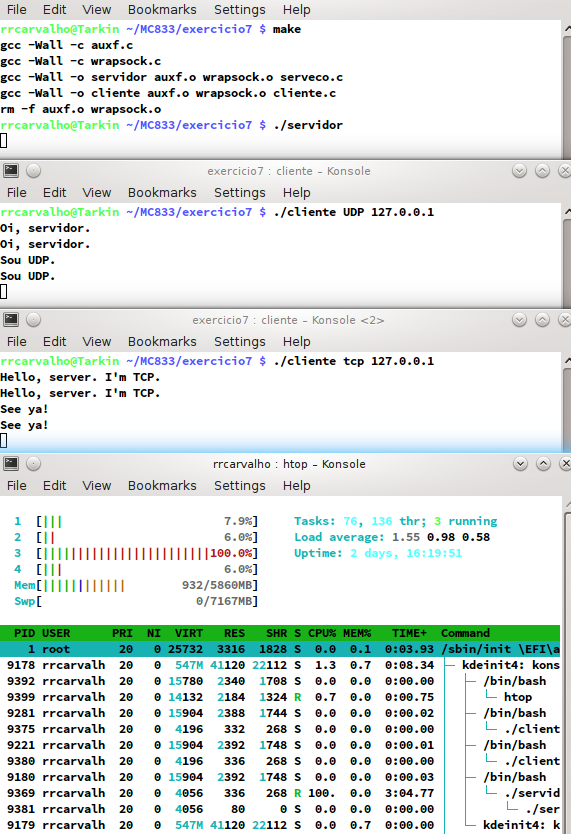
\includegraphics[width=117mm]{images/teste.png}
  \label{teste}
\end{figure}
\paragraph{}Além do teste da figura. Foram testados múltiplos clientes TCP e múltiplos clientes UDP com sucesso. Finalmente, um último teste entre um laptop rodando ArchLinux e uma máquina virtual Linux Mint foi feito em uma rede local (LAN), também com sucesso.



\end{document}
